One of the hardest part of creating and training \gls{ml} models is accurately evaluating their performance. How can you known if your model is giving out accurate predictions ? What is accuracy, and how can we precisely define it ? Understanding the types of errors a detection model can make is a crucial part in enhancing their performance. In this section, we will present metrics used in detection and classification tasks that can help us to evaluate and understand how and where a given model succeed and fail.

\section{Type of Errors}
In a classification task, where a model is asked to classify an item into a fixed number of categories based on input characteristics, a model will predict the class of a given item. For example if an input image contains a cat or a dog. In doing so, the model can make mistakes. When predicting a particular class, there are 2 type of predictions that can be made: positive or negative, and those predictions can be true or false. When a network correctly predicts that an image contains a cat, it is a true positive. When it predicts that there is no dog when there is one, this is a false negative.

All in all, there are 4 categories of predictions: True Positive (TP), False Positive (FP), True Negative (TN) and False Negative (TN). 

\section{Precision and Recall}
Precision is defined as "the fraction of detections reported by model that were correct" and recall is "the fraction of detections reported by the model which were correct"\cite[p.411]{Goodfellow2016}. We can see those concepts visualised in Figure~\ref{fig:precRecall}. In that Figure, the precision would be equal to the number True Positives in green divided by number of selected elements \textit{i.e.} the green and red sets combined. The recall would be equal to the number of true positives over the total number of relevant elements or the dark gray set and the green set combined. 

\begin{figure}[h]
  \centering
  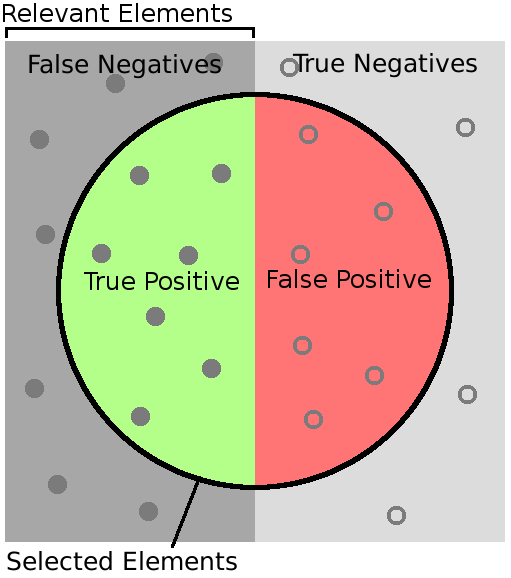
\includegraphics[width=0.7\textwidth]{precisionRecall}
	\caption[]{Precision and recall on a classification task. Figure adapted from Wikipedia\cite{precRecall}}
  \label{fig:precRecall}
\end{figure}

Precision and recall allows us to quantify with more accuracy the quality of a model than just the number of errors that it makes. For example, in the case of a model trying to detect a rare event like a disease that would infect only a small fraction of the population, say one in a million, \textbf{a detector that would always infer that a person is not sick would be able to attain a $99.9999\%$ accuracy.} However, while this detector would achieve a very high precision, it would have a very bad recall, which would indicate that it is not a very good model after all.

\section{Intersection over Union (IoU)}\label{iouExplanation}
The intersection over union, or Jaccard Index quantifies the accuracy of the bounding box prediction. \gls{iou} measure the quality of a bounding box : if the predicted bounding box overlaps significantly with the ground truth bounding box, then it should have a low score, and inversely if the prediction does not overlap with the ground truth. The \gls{iou} is given by the following equation:

\begin{equation}
	IoU = \frac{\text{area}(BBox_{truth} \cap BBox_{pred})} {\text{area}(BBox_{truth} \cup BBox_{pred})}
\end{equation}

\begin{figure}
  \centering
  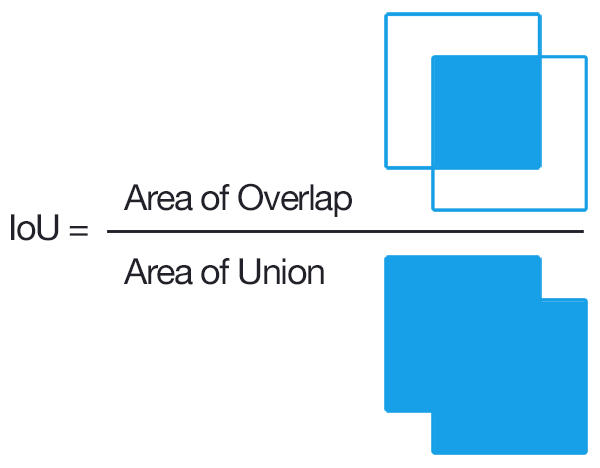
\includegraphics[width=0.5\textwidth]{iou}
	\caption[Intersection over Union]{Intersection over Union\\\textbf{Source}: https://www.pyimagesearch.com/2016/11/07/intersection-over-union-iou-for-object-detection/}
  \label{fig:iou}
\end{figure}

Generally a detection is considered correct if the $\text{IoU} \geq 0.5$; this threshold is also used when computing the \gls{map}. It should also be noted that the \gls{iou} is not the only way to measure how good a bounding box is. Improvements on this metric has been done that gives out a better measure on the quality of the box, such as the \gls{giou}\cite{giou}, \gls{diou}\cite{diou} and \gls{ciou}\cite{diou}. Those metrics are used in our model, and are presented in Section~\ref{ious}. 

\section{F1-Score, Average Precision and Mean Average Precision (mAP)}
The F1-Score is a measure of test accuracy. It is the harmonic mean of precision and recall :
\begin{equation}
	2 \cdot \frac{precision \cdot recall}{precision + recall}
\end{equation}

The Average Precision (AP) is a popular metric used to measure the accuracy of object detector. In this section, we will use the example of a model asked to detect a single class of object, like a dog. In total, there are 5 dogs in the dataset. 

To compute the AP, one first draws a list of all predictions made by the model, and rank it according to the predicted confidence level. As we go down the list, the recall value will increase, as it is the proportion of TP over all possible positives. Precision will have a "zig-zag" pattern, where it will go up with TP but down with FP. The AP is defined as the area under this curve, or:
\begin{equation}
	AP = \int_0^1 p(r) dr
\end{equation}
Where $p(r)$ is the precision of the model according to a given recall value. Since precision and recall are always between 0 and 1, AP will also be between 0 and 1. 

The COCO \gls{map}, or mAP@50 is simply the AP average over all classes for \gls{iou} that are over 0.5. Sometimes, different values of the \gls{map} are given for different values of the \gls{iou} required to have a successful detection.

The mean average precision is the metric used by the COCO dataset\cite{msCOCO}. As said above, when the \gls{iou} between the prediction and the ground truth is over 0.5, the prediction is considered a valid detection. 


\section{Confusion Matrices}
\begin{table}[H]
	\centering
	\begin{tabular}{ll|cc}
		                           &   & \multicolumn{1}{l}{} & \multicolumn{1}{l}{Predictions} \\ \cline{3-4} 
					                              &   & P                    & N                               \\ \hline
								      \multicolumn{1}{l|}{}      & P & TP                   & FN                              \\
								      \multicolumn{1}{l|}{Truth} & N & FP                   & TN                             
	\end{tabular}
	\caption{Abstract representation of a confusion matrix. If the prediction is the same as the ground truth, then the prediction is a True Positive/Negative (TP/TN). If it is not, it is a False Positive/Negative (FP/FN) }
	\label{tab:confusionMatAbs}
\end{table}
	
This metric is a very popular way of seeing how a model fails to classify objects, in particular how it confuses classes. A confusion matrix is a $N \times N$ matrix, with $N$ being the number of classes. Each row represents the instance in a predicted class, while each column represents the predicted instance.\cite{powerDavid2008}. A perfect model would give a diagonal matrix, where each prediction match with the label. 

\begin{table}[H]
	\centering
	\begin{tabular}{ll|ccc}
		                           &      & \multicolumn{1}{l}{} & \multicolumn{1}{l}{Predictions} & \multicolumn{1}{l}{} \\ \cline{3-5} 
					                              &      & Cat                  & Lion                            & Dog                  \\ \hline
								      \multicolumn{1}{l|}{}      & Cat  & 12                   & 6                               & 1                    \\
								      \multicolumn{1}{l|}{Truth} & Lion & 7                    & 8                               & 0                    \\
								      \multicolumn{1}{l|}{}      & Dog  & 0                    & 1                               & 14                  
	\end{tabular}
	\caption{Example of a confusion matrix. Here, we can easily see that the model often confuses Lion and Cat, but the Dog class is not being confused much for any other class.}
	\label{tab:confusionMat}
\end{table}

Table~\ref{tab:confusionMat} shows an example of a confusion matrix for a model predicted 3 classes. In the case of an object detector, where the model outputs bounding box which can be anywhere in an input image, a prediction is considered only when the \gls{iou} of the box and the ground truth is over 0.5. Predictions matrices are also usually normalised.
\section{Matthews Correlation Coefficient}%TODO
The \gls{mcc} is a metric often used in bioinformatics to measure the quality of binary class predictions, and takes into account true and false positive. The \gls{mcc} has been introduced by Matthews in 1975, and is a correlation coefficient between prediction and ground truth.\cite{matthews1975} The \gls{mcc} is regarded as a more balanced metric than the F1-Score\cite{chicco2020}\cite{luque2020} and has seen some recent use in archaeological object detection. The \gls{mcc} can be used with classes of very different size, and returns a value between -1 and 1. A score of -1 means complete disagrement between predictions and truth, 0 indicates that the predictions are not better than a random choice of class, and 1 indicates that a perfect prediction.

The \gls{mcc} is regarded as one of the best way to describe a confusion matrix using a single number, and is defined as follow:

\begin{equation}
	MCC = \frac{TP \times TN - FP \times FN}{\sqrt{(TP + FP)(TP + FN)(TN + FP)(TN + FN)}}
\end{equation}

In the case of multi class prediction, the formula is slightly more complicated, and is defined in terms of a $K \times K$ confusion matrix, and $C$ classes\cite{gorodkin2004}:


\begin{equation}
	MCC = \frac{\sum_k \sum_l \sum_m C_{kk} C_{lm} - C_{kl}C_{mk}}
	{\sqrt{\sum_k (\sum_l C_{kl})(\sum_{k'|k \neq k'} \sum_{l'}C_{k'l'})}
	\sqrt{\sum_k (\sum_l C_{lk})(\sum_{k'|k \neq k'} \sum_{l'}C_{l'k'}})}
\end{equation}
\section{Evaluating a model}
Computing those metrics and analyzing them allows a researcher to better understand the behavior of its model, and preventing degenerate behavior. It should however be noted that those metrics do not always give out accurate or useful information. In that case, only knowledge and experience of the usual issues can help.

For example, it can happen that a model will always infer one class other another, for any kind of object and still obtain good accuracy\footnote{This often happens in the case of an unbalanced dataset, where one class appear more often than any other.}. It can also be the case that a metric is very sensible at a some scale of errors but not at others: the L2 distance for example grows quadratically and outputs small distances when the L1 distance is below 1, but very high values that might be hard to optimize for when the L1 distance is over 1.

The only way to diagnose those issues will be to manually inspect the prediction of the model, and carefully choosing the metrics used. 

